%!TEX TS-program = xelatex
%!TEX encoding = UTF-8 Unicode

% TAMAGOTCHI
% - - - - - - - - - - - - - - - - - - - - - - - - - - - - - - - - - - - - - -

\documentclass[
	12pt,
	a5paper,
	twoside,
	openany,
	titlepage
	]{book}

\usepackage[
	top=2.0cm,
	bottom=2.5cm,
	inner=2.0cm,
	outer=2.0cm,
%	textheight=16cm,
	heightrounded
	]{geometry}

\widowpenalty10000
\clubpenalty10000
\parskip=0.0em
%\parindent=5mm
\usepackage{indentfirst}

% lineas huérfanas y viudas
	\clubpenalty=10000
	\widowpenalty=10000

% interlineado
\usepackage{setspace}
	\linespread{1.25}

% % % % % % % % % % % % % % % % % % 

% LISTAS, TABLAS Y COLUMNAS
\usepackage[ampersand]{easylist}
\usepackage{paralist}	% listas dentro de los párrafos
\usepackage{enumitem}
	\setenumerate{
		label={\arabic*.},
		ref={\arabic*},
		itemsep=0.0\baselineskip,
		topsep=0.5\baselineskip,
		leftmargin=1.0cm
		}
	\setitemize{
		label={--},
		itemsep=0.0\baselineskip,
		topsep=0.5\baselineskip,
		leftmargin=1.0cm
		}
	\newlist{linelist}{enumerate*}{1}
		\setlist[linelist]{label={(\roman*)}}
\usepackage{longtable}	% tablas extensas
\usepackage{multicol}
	\setlength\columnsep{1.0cm}

% UTILIDADES
\usepackage{etoolbox}	% navaja suiza
\usepackage{calc}		% operaciones matemáticas sencillas
\usepackage{ifthen} 	% condicional programable
\usepackage{blindtext}	% texto de maquetación
\usepackage{lastpage}	% detectar última página
\usepackage{datetime}	% manejo avanzado de fechas
%\usepackage{showframe}	% muestra los bordes de la página
						% da problemas con xcolor

% IDIOMA, LOCALIZACIÓN
\usepackage[spanish]{babel}
\usepackage[autostyle=true]{csquotes}	% comportamiento comillas

% GRÁFICOS Y COLORES
\usepackage{graphicx}
	\DeclareGraphicsExtensions{.pdf,.png,.jpg,.eps}
	\graphicspath{{img/}}
\usepackage[usenames,dvipsnames]{xcolor}

% IMÁGENES Y FIGURAS
\usepackage{wrapfig}	% emplazamiento especial
\usepackage{caption}	% pie de figura
%\usepackage{subcaption}	% pie de figura para subdivididas
%\usepackage{subfig}		% subdivisión de figuras

% TEXTO A BANDERA
\usepackage{ragged2e}

% GLOSARIO E ÍNDICES ALFABÉTICOS
\usepackage{imakeidx}
	\makeindex[intoc,name=princ,title=\textbf{Índice alfabético general}]
	\makeindex[intoc,name=gente,title=\textbf{Índice onomástico}]
\makeindex 

% TITULOS
%\usepackage{titletoc}
\usepackage{titlesec}
	\titleformat{\chapter}[block]
		{\sffamily}
		{[\chaptertitlename\thechapter]}
		{-50pt}
		{\newline\bfseries\Large\sffamily}

\titlespacing*{\chapter}{0cm}{2.5cm}{1cm}

% TIPOGRAFÍAS Y MOTOR
\usepackage{fontspec}
	\usepackage{xltxtra}
	\usepackage{xunicode}
\defaultfontfeatures{
%	Ligatures={Rare,Historical},
%	Style=Historic,
	Kerning=On,
	Style=TitlingCaps,
	Mapping=tex-text % ligadura de los guiones
	}

\setromanfont{EB Garamond}
\setsansfont{DejaVu Sans}
\setmonofont{DejaVu Sans Mono}

%\newfontfamily⟨cmd⟩{⟨font name⟩}[⟨font features⟩]
\newfontfamily\medieval{Essays1743}

% TIPOGRAFÍAS ESPECIALES
\usepackage{alltt}		% input «as is» ; permite \emph{}
\usepackage{fancyvrb}	% input «as is» extras
\usepackage{amsfonts}	% matemáticas
\usepackage{amssymb}	% símbolos varios
\usepackage{amsmath}	% matemáticas
%\usepackage{arev}		% griego y cirílico
\usepackage{marvosym}	% símbolos y emoticonos

% COMPORTAMIENTOS ESPECIALES
\usepackage{colonequals}

% NOTAS
%\usepackage{marginnote}
%\usepackage{endnotes}
\usepackage[hang,flushmargin,bottom,perpage]{footmisc} 
\usepackage{dblfnote}

\renewcommand\thefootnote{\arabic{footnote}}
\renewcommand\footnoterule{}
\setlength{\skip\footins}{0.25cm}
\setlength{\footnotesep}{1.0\baselineskip}

% PROGRAMACIÓN CAPÍTULO
% para poder emplearlo en los encabezados
\newcommand{\capitulo}[1]{%
	\clearpage%
	\def\nombrecap{#1}%
	\chapter{#1}%
}

% ESTILOS DE PÁGINA
\usepackage{fancyhdr}
	\pagestyle{empty}
	\assignpagestyle{\chapter}{capitexto}
	\addto\captionsspanish{%
		\renewcommand\chaptername{Txt.}
	}

% diseño general de la páginas
\fancypagestyle{plain}{
	\fancyhf{}
	\fancyhf[HCEO]{%
	{\ttfamily\scriptsize\MakeUppercase\nombrecap}
	}
	\fancyhf[HLO]{}
	\fancyhf[FLE]{%
	{\ttfamily\footnotesize\thepage\dots}
	}
	\fancyhf[FRE]{%
	{\ttfamily\scriptsize WE ARE}
	}
	\fancyhf[FLO]{%
	{\ttfamily\scriptsize TAMAGOTCHI}
	}
	\fancyhf[FRO]{%
	{\ttfamily\footnotesize\dots\thepage}
	}
	\renewcommand{\headrulewidth}{0.5pt}
	\renewcommand{\footrulewidth}{0.5pt}
}

% diseño particular del capítulo
\fancypagestyle{capitexto}{
	\fancyhf{}
	\fancyhf[HCEO]{~}
	\fancyhf[HLO]{}
	\fancyhf[FLE]{%
	{\ttfamily\footnotesize\thepage\dots}
	}
	\fancyhf[FRE]{%
	{\ttfamily\scriptsize WE ARE}
	}
	\fancyhf[FLO]{%
	{\ttfamily\scriptsize TAMAGOTCHI}
	}
	\fancyhf[FRO]{%
	{\ttfamily\footnotesize\dots\thepage}
	}
	\renewcommand{\headrulewidth}{0.5pt}
	\renewcommand{\footrulewidth}{0.5pt}
}

\pagestyle{plain}

% BIBLIOGRAFIA
% hay que compilar 4 veces: [ latex, bibtex, latex, latex ]
\usepackage{cite}
\usepackage{chicago}
\addto\captionsspanish{%
	\renewcommand\bibname{Referencias}}

% ENLACES E INFO PDF
	% este paquete tiene que ser el último en cargar
\usepackage[hidelinks]{hyperref}
	\hypersetup
	{
	pdfauthor={TAMAGOTCHI},
	pdfsubject={TEXTOS},
	pdftitle={TAMAGOTCHI},
	pdfkeywords={tags},
	pdfdisplaydoctitle={true}
	}
	\providecommand\phantomsection{}

% - - - - - - - - - - - - - - - - - - - - - - - - - - - - - - - - - - - - - -

\title{\textbf{\sffamily ONTOLOGÍA}}
\author{\sffamily TAMAGOTCHI}
\date{\sffamily\textbf{[ 01 ]}}

\begin{document}
%\maketitle
%!TEX root = ../index.tex
% - - - - - - - - - - - - - - - - - - - - - - - - - - - - - - - - - - - -

\begin{titlepage}
\centering

\settowidth{\unitlength}{\LARGE WE ARE TAMAGOTCHI}

\vspace*{\baselineskip}

{\Large\scshape tamagotchi}\\[\baselineskip]

\rule{\unitlength}{1.6pt}\vspace*{-\baselineskip}\vspace*{2pt}
\rule{\unitlength}{0.4pt}\\[\baselineskip]

{\LARGE I}\\[\baselineskip]

{\itshape título}\\[0.2\baselineskip]

\rule{\unitlength}{0.4pt}\vspace*{-\baselineskip}\vspace{3.2pt}
\rule{\unitlength}{1.6pt}\\[\baselineskip]

{\large\scshape \today}\par

\vfill

{\large\scshape wearetamagotchi.com}\\[\baselineskip]
{\small\scshape (CC):BY-SA 4.0}\par

\end{titlepage}
%%!TEX root = ../index.tex
% - - - - - - - - - - - - - - - - - - - - - - - - - - - - - - - - - - - -
\thispagestyle{empty}
\begin{Verbatim}[fontsize=\scriptsize]
MMMMMMMMMMMMMMMMMMMMMMMMMMMMMMMMMMMMMMMMMMMMMMMMMMMMMMMMMMMMMMMM
MMMMMMMMMMMMMMMMMMMMMMMMMMMWNK0OO0KXWMMMMMMMMMMMMMMMMMMMMMMMMMMM
MMMMMMMMMMMMMMMMMMMMMMXkl;.          .;lkXMMMMMMMMMMMMMMMMMMMMMM
MMMMMMMMMMMMMMMMMMWO:.                    .cOWMMMMMMMMMMMMMMMMMM
MMMMMMMMMMMMMMMM0:           .,::;'.          :0MMMMMMMMMMMMMMMM
MMMMMMMMMMMMMWx.           'oddddddo:           .xWMMMMMMMMMMMMM
MMMMMMMMMMMWx.             oddddddddd'            .xWMMMMMMMMMMM
MMMMMMMMMM0.               :odddddddl.              .OMMMMMMMMMM
MMMMMMMMWc                  .;cllc:'                  :NMMMMMMMM
MMMMMMMN'                                              .XMMMMMMM
MMMMMMX.                                                .KMMMMMM
MMMMMN.                                                  .KMMMMM
MMMMW,            :OKXXXXXXXXXXXXXXXXXXXXXXX0d.           .NMMMM
MMMMd            'XXXXXXXXXXXXXXXXXXXXXXXXXXXXd            cMMMM
MMMW.            ,XXXXXXXXXXXXXXXXXXXXXXXXXXXXd             XMMM
MMMO             ,XXXXXXXXKccOXXXXXXlc0XXXXXXXd             oMMM
MMMo             ,XXXXXXXXKccccxXXXXlcccdXXXXXd             ;MMM
MMMc             ,XXXXXXXXXXXdcccoXXXXdc:clXXXd             ,MMM
MMMl             ,XXXXXXXXXXXo;:coXXXXo;:clXXXd             ;MMM
MMMx             ,XXXXXXXXKlcccxXXXXocccxXXXXXd             lMMM
MMMX             ,XXXXXX0cc::kXXX0cc::OXXXXXXXd             OMMM
MMMM:            ,XXXXXX0clKXXXXX0cc0XXXXXXXXXd            'WMMM
MMMMX            ,XXXXXXXXXXXXXXXXXXXXXXXXXXXXd            kMMMM
MMMMMd           .OXXXXXXXXXXXXXXXXXXXXXXXXXXK;           cMMMMM
MMMMMMl            .,;;;;;;;;;;;;;;;;;;;;;;;'            ,WMMMMM
MMMMMMMl                                                ,WMMMMMM
MMMMMMMMo           .;;;;.   .,;;;.   ,;;;,.           :WMMMMMMM
MMMMMMMMMO.          ....     ....    .....           xMMMMMMMMM
MMMMMMMMMMWl                                        :NMMMMMMMMMM
MMMMMMMMMMMMXl                                    :KMMMMMMMMMMMM
MMMMMMMMMMMMMMNd'                              .lXMMMMMMMMMMMMMM
MMMMMMMMMMMMMMMMMXd,                        'lKMMMMMMMMMMMMMMMMM
MMMMMMMMMMMMMMMMMMMMNOo:'.             .;lkNMMMMMMMMMMMMMMMMMMMM
MMMMMMMMMMMMMMMMMMMMMMMMMMNK0OkkkkO0KNMMMMMMMMMMMMMMMMMMMMMMMMMM
MMMMMMMMMMMMMMMMMMMMMMMMMMMMMMMMMMMMMMMMMMMMMMMMMMMMMMMMMMMMMMMM
MMMMMMMMMMMMMMMMMMMMMMMMMMMMMMMMMMMMMMMMMMMMMMMMMMMMMMMMMMMMMMMM
\end{Verbatim}
%\clearpage
%!TEX root = ../index.tex
% - - - - - - - - - - - - - - - - - - - - - - - - - - - - - - - - - - - -

\thispagestyle{empty}

\sffamily\vspace*{\fill}

\begin{flushright}\footnotesize
[+ info]\linebreak
\url{http://wearetamagotchi.com}
\end{flushright}

\rmfamily

% no imprimir para el fanzine
%\setcounter{tocdepth}{1}
%\tableofcontents

\setcounter{page}{1}
%!TEX root = ../index.tex
% - - - - - - - - - - - - - - - - - - - - - - - - - - - - - - - - - - - -

%!TEX root = ../index.tex
% - - - - - - - - - - - - - - - - - - - - - - - - - - - - - - - - - - - -

\capitulo{El comienzo}

Este texto es para probar las ligaduras.

\begin{wrapfigure}[5]{r}[-0.25cm]{2.0cm}
	\vspace{-0.5\baselineskip}
	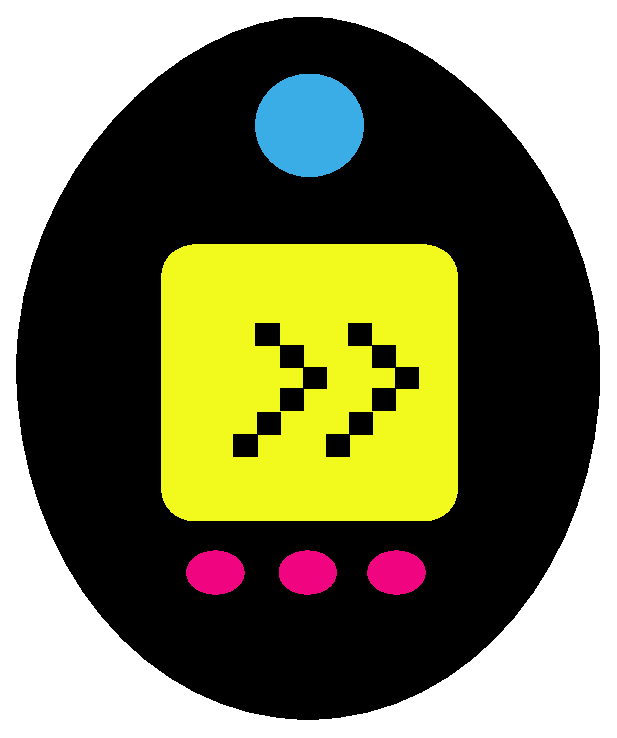
\includegraphics[width=2.0cm]{logo_cl}
\end{wrapfigure}

\Blindtext




%\clearpage
%\setcounter{chapter}{0}
%\def\nombrecap{}
%\printindex[princ]
%\printindex[gente]

%\bibliographystyle{chicago}	% plain, unsrt, alpha, abbrv
%\bibliography{biblio/bibprincipal}
% -- o --
%%!TEX root = ../index.tex
% - - - - - - - - - - - - - - - - - - - - - - - - - - - - - - - - - - - -

\begin{thebibliography}{9}
\bibitem{libro1}
	Leslie Lamport,
	\textit{\LaTeX: a document preparation system},
	Addison Wesley, Massachusetts,
	2nd edition,
	1994.
\end{thebibliography}

%!TEX root = ../index.tex
% - - - - - - - - - - - - - - - - - - - - - - - - - - - - - - - - - - - -

\clearpage
\thispagestyle{empty}
\vspace*{\fill}
\noindent
\begin{center}
	\scshape\large
	[ \today\ ]
	\vspace{0.5cm}
	\par
	\noindent
	* * *
\end{center}
\vspace*{\fill}
\end{document}

% - - - - - - - - - - - - - - - - - - - - - - - - - - - - - - - - - - - - - -
% FIN DEL ARCHIVO